\chapter{Studiu bibliografic/Stadiul actual în domeniu}

În cadrul acestei secțiuni, vom prezenta câteva dintre soluțiile deja existente pentru a 
distribui sarcina de compilare a unui proiect asupra mai multor sisteme de calcul ce comunică
prin intermediul unei rețele.

\section{Distcc}

\textbf{Distcc}\cite{pool2003distcc} oferă posibilitatea de a distribui sarcina de compilare între
mai multe sisteme ce comunică în rețea, fără a fi nevoie ca sistemele participante să partajeze 
același sistem de fișiere, fără sincronizare de clock-uri sau să aibă acces la aceeași versiune a
codului sursă. 

Distcc funcționează prin distribuirea sarcinilor de lucru de la un sistem client, către nodurile
server, care vor realiza compilarea. Inițial, se analizează comanda de compileare executată de
către client, pentru a determina dacă sarcina poate fi distribuită, se aleg nodurile care să
deservească cererea, apoi se rulează local preprocesorul asupra fișierelor ce vor fi supuse
compilării. Ulterior, nodurile server primesc request-uri ce conțin fișierele sursă preprocesate și
returnează către client fișierele obiect rezultate în urma compilării sau o listă cu erorile de 
compilare, în cazul unui eșec.

Aplicația client este invocată ca un wrapper pentru compilator-ul obișnuit (GCC de obicei), de către
script-urile de build rulate de \textbf{GNU Make}. Comunicare între client-ul Distcc și nodurile
server se realizează prin protocoalele de rețea \textbf{TCP} sau \textbf{SSH}, folosind un set
simplu de mesaje pentru a trimite cereri de compilare: mesajul pentru cerere conține versiunea de
protocol utilizată, argumentele din linia de comandă pentru invocarea compilatorului și fișierele
sursă, în timp ce răspunusl unui nod server returnează fișierele obiect aferente.

Distcc oferă posibiliteate ca mesajele interschimbate între nodurile client și server să fie
comprimate înainte de trimitere, pentru a reduce dimensiune volumui de date trimis, folosind
metoda de comprimare \textbf{LZO}\cite{tarreau2018lzo}, care se concentrează asupra obținerii unei 
viteze cât mai bune pentru operația de decompresie. Micșorarea volumui de date folosind compresia,
îmbunătățește throughput-ul de cereri transmise între participanții sistemului Distcc.

Planificarea pentru lansarea noilor sarcini de compilare folosește un mecanism simplu, prin care
fiecare participant păstrează un fișier de stare, iar suprasolicitarea unui nod este împiedicată
prin definirea unui număr limită de job-uri de compilare care pot fi soluționate simultan, care
ia o valoare dependentă de numărul de procesoare fizice de care dispune fiecare nod. La
inițializare, fiecare nod pornește numărul maxim de procese Distcc-server, care ulterior așteaptă
inițierea unei conexiuni de către un client care va solicita compilarea. Pentru a putea coordona
activitatea proceselor server care rulează simultan pe fiecare nod, se folosesc fișiere lock Unix,
care sunt eliberate automat de către un proces în momentul terminării sale.

Un dezavantaj al sistemului distribuit Distcc îl constituie faptul că nu există niciun mecanism
de estimare a timpului de compilare pentru un nod, deoarece această valoarea nu este dependentă
doar de dimensiunea codului sursă, ci și de aspecte precum complexitatea codului sursă sau 
specificațiile hardware ale nodului respectiv. Așadar, pătrunderea unui nod foarte lent în rețeaua
de servere Distcc, poate încetini semnificativ procesul de build, deoarece nodul solicitant va trebui
să aștepte ca fiecare nod server să își finalizeze sarcina, înainte de a primi fișierele obiect și
de a invoca linker-ul.

Totodată, un inconvenient care nu trebuie neglijat este faptul că Distcc este o aplicație care 
rulează exclusiv pentru sisteme de operare de tip \textbf{Linux}, ceea ce nu rezolvă problema
compilării distribuite pentru \textbf{Windows}.

La data prezentării inițiale a Distcc, autorul afirmă că micșorarea timpilor de build este
o valoare ce se modifică liniar, odată cu numărul de core-uri de procesare implicate, cel puțin
pentru un număr mic de core-uri (pentru 3 calculatoarele, build-ul a fost de 2.8 ori mai rapid). În
ceea ce privește scalabilitatea sistemului Distcc, trebuie luat în calcul că dintre toate sarcinile
aferente procesului de build: execuție Makefile, preprocesare, compilare, linking, doar compilarea
este distribuită la mai multe noduri \cite{ashby2004parallel}. Pentru a determina care este limita
de paralelizare a procesului de build, trebuie consultată Legea lui Amdahl, vizibilă în Figura
\ref{fig:amdahl}:

\begin{figure}[H]
    \centering
    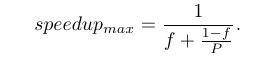
\includegraphics[width=0.43\linewidth, height=0.17\linewidth]{figures/amdahl.jpg}
    \caption{Legea lui Amdahl}
    \label{fig:amdahl}
\end{figure}

Chiar dacă numărul de procesoare \textbf{P} tinde spre infinit, aportul de performanță
este limitat de porțiunea din proces ce nu poate fi paralelizată \cite{ashby2004parallel}.

Figura \ref{fig:distcc} exemplifică modul de funcționare al Distcc.

\begin{figure}[H]
    \centering
    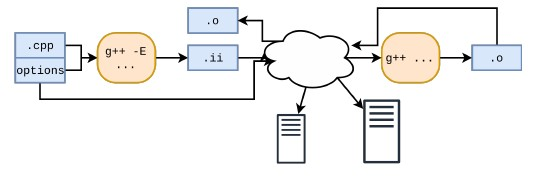
\includegraphics[width=0.63\linewidth, height=0.37\linewidth]{figures/distcc.jpg}
    \caption{Funcționarea Distcc \cite{matev2020fast}}
    \label{fig:distcc}
\end{figure}

\section{Ccache}

Deși nu reprezintă un sistem distribuit, \textbf{Ccache}\cite{ccache} este un mecanism caching pentru
rezultatul compilării de fișiere sursă foarte des folosit alături de metoda descrisă anterior, 
Distcc, pentru a micșora și mai mult durata de build distribuit. Această combinație dintre 
\textbf{Distcc} și \textbf{Ccache} a fost studiată atent la Institutul CERN\cite{matev2020fast},
întrucât procesul de build inițial pentru un proiect poate ajunge la 5 ore.

Sistemele tradiționale de build, precum \textbf{GNU Make} și \textbf{Ninja}, analizează timestamp-ul
ultimei modificări a unui fișier sursă pentru a determina daca compilatorul va fi invocat asupra
unui fișisier sursă sau nu. Problema apare în momentul schimbării de branch pentru sisteme de 
versionare precum \textbf{Git}, întrucât timestamp-ul fișierelor sursă își actualizează valoarea
chiar dacă, conținutul nu se modifică, evenimentul fiind de natură să determine o recompilare
completă a întregului proiect.

O proprietate interesantă a procesului de build pentru limbajele \textbf{C/C++} o constituie faptul
că output-ul este complet determinat de conținutul surselor preproceesate și de argumentele de rulare
ale compilatorului. Această proprietate este utilizată de către Ccache pentru a stoca output-ul
compilării pentru un anumit fișier sursă, iar mai apoi să îl redea, în momentul începerii unui
nou proces de build, evitând astfel apelarea inutilă a compilatorului pentru un fișier ce nu a
fost modificat.

Sarcina principală pe care Ccache o îndeplinește o reprezintă determinarea existenței unui fișier
object file asociat fișierului sursă de intrare, prin calcularea unei valori de dispersie bazată
pe conținutul fișierului sursă și a flag-urilor folosite la compilarea inițială. 

Ccache suportă mai multe moduri de operare, cel mai simplu dintre acestea fiind numit 
\textbf{preprocessor mode}, care presupune rularea preprocesorului asupra fișierului sursă
de intrare, iar mai apoi calcularea valorii hash pe baza conținutului unității de translație
rezultate \cite{ccache_manual}. Dezavantajul acestui mod de funcționare este necesitatea de
a apela întotdeauna preprocesorul asupra fișierului sursă de intrare, ceea ce încetinește
lookup-ul.

\begin{figure}[H]
    \centering
    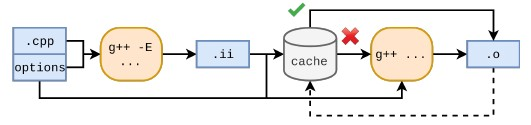
\includegraphics[width=0.63\linewidth, height=0.27\linewidth]{figures/ccache_direct.jpg}
    \caption{Ccache preprocessor mode \cite{matev2020fast}}
    \label{fig:ccache_pre}
\end{figure}

De asemenea, Ccache poate funcționa într-un mod care evită pe cât posibil rularea preprocesorului,
această acțiune fiind realizată doar în eventualitatea unui \textbf{cache miss}. În cadrul acestui
mod de operare, valoarea hash este calculată direct pe baza fișierului sursă, fără preprocesare,
iar valoarea este inclusă în cadrul unui fișier \textbf{manifest}, care conține referințe către
rezultatele precedente al compilării (fișiere obiect, dependințe), care au fost produse pentru
același hash, căi către fișierele header accesate la timpul compilării și valori checksum pentru
fișierele incluse. În cazul unui cache miss, este necesară recalcularea valorii hash pentru fișierul
de intrare și actualizarea manifest-ului.

\begin{figure}[H]
    \centering
    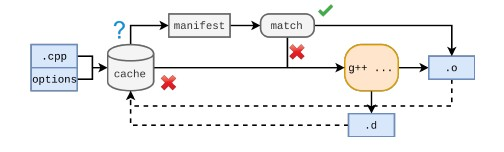
\includegraphics[width=0.63\linewidth, height=0.32\linewidth]{figures/ccache_pre.jpg}
    \caption{Ccache direct mode \cite{matev2020fast}}
    \label{fig:ccache_direct}
\end{figure}

În cazul folosirii Ccache împreună cu sistemul distribuit Distcc, apare problema evidentă: cache-ul
de compilare nu este distribuit pentru toate nodurile rețelei, ci fiecare nod participant are acces
doar la cache-ul său local.

\newpage

\section{Sccache}

Sscache\cite{sccache} reprezintă varianta distribuită ca sistemului Ccache, care adaptează cache-ul
inițial pentru a putea fi găzduit în cadrul unui serviciu cloud (sau pur și simplu remote) de stocare, precum: Amazon S3, Redis sau Cloudflare R2, ceea ce soluționează nevoia ca fiecare nod 
participant la procesul de compilare să dețină un cache local de fișiere obiect, care conține 
înregistrări doar pentru datele de intrare prelucrate de nodul respectiv.

Această soluție oferă un mecanism wrapper peste Ccache, astfel încât accesul la datele stocate remote
să fie reglementat într-o manieră client-server \cite{saario2020enabling}. Spre deosebire de Ccache,
pentru calcularea unei valori hash se invocă întotdeauna preprocesorul, având astfel un comportament
similar cu modul de operare \textbf{preprocessor mode}, dar se face offloading pentru volumul de 
date.

\section{DiSCo}

Dacă în cazul utilizării Distcc, singura dintre sarcinile din procesul de build care este 
paralelizată, este invocarea compilatorului asupra fișierelor preprocesate, \textbf{DiSCo}
\cite{jo2013disco} propune o abordare inedită, în care preprocesarea, compilarea și 
link-editarea sunt efectuate în mod paralel, utilizând noduri remote.

Distcc utilizează schema de preprocesare locală, mult mai rudimentară, prin care nodul care
solicită compilarea este singurul responsabil pentru realizarea etapei. Întrucât toată operațiunea
are loc local, nu există problema ca un fișier de intrare să nu fie valabil, însă impune un cost
însemnat asupra scalabilității sistemului. Pe de altă parte, preprocesarea remote, abordare aleasă
de \textbf{DiSCo}, micșorează durata preprocesării, însă volumul de date tranzacționat între 
nodurile sistemului este mai mare, deoarece nu se mai trimite prin rețea doar fișiserul preprocesat,
ci atât fișierul sursă, cât și toate fișierele header asociate. O abordare asemănătoare adoptă și
sistemul \textbf{IncrediBuild}\cite{incredibuild}, despre care nu sunt cunoscute multe 
detalii de funcționare, întrucât este o soluție comercială.

În ceea ce privește arhitectura sistemului de compilare distribuită \textbf{DiSCo}, la baza acestuia
se află o serie de mai multe componente:

\begin{itemize}
    \item Command Scheduler - modul care parsează conținutul unui \textbf{Makefile} pentru a determina potențialele dependințe dintre comenzile individuale de compilare, iar în funcție
    de relația dintre aceste comenzi, entitățile independente sunt grupate în blocuri de comenzi,
    elementele unui bloc fiind executate în paralel, iar mai multe blocuri de comenzi consecutive
    sunt executate secvențial; totodată, modulul command scheduler folosește o metodă de planificare
    statică pentru a determina spre ce nod al sistemului să fie trimis un anumit bloc de comenzi
    \item Connection Manager - folosește un mecanism de tip thread pool pentru a deschide sau termina
    conexiuni cu nodurile adiacente, folosite pentru comunicarea statusului pentru un proces de 
    compilare în desfășurare \cite{mizuno2003synchronization}
    \item Compilation Manager - modul responsabil pentru executarea etapelor procesului de
    compilare
    \item Network Drive Manager - gestionează transferul de fișiere în mod implicit între nodurile
    sistemului și mediază interacțiunea cu \textbf{H-Cache-ul} nodului, responsabil pentru stocarea
    eficientă de fișiere header
\end{itemize}

Figura \ref{fig:disco} ilustrează arhitectura sistemului distribuit de compilare DiSCo.

\begin{figure}[H]
    \centering
    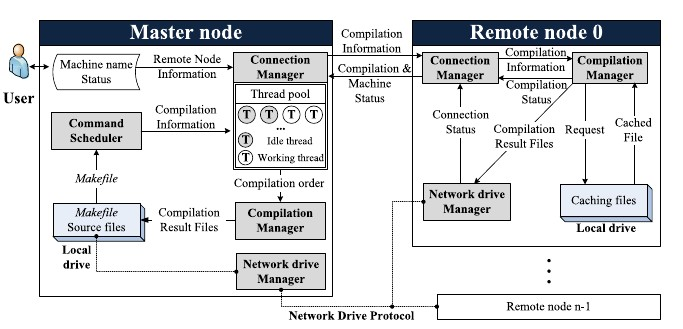
\includegraphics[width=0.83\linewidth, height=0.5\linewidth]{figures/disco.jpg}
    \caption{Arhitectura Disco \cite{jo2013disco}}
    \label{fig:disco}
\end{figure}